% Template for PLoS
% Version 1.0 January 2009
%
% To compile to pdf, run:
% latex plos.template
% bibtex plos.template
% latex plos.template
% latex plos.template
% dvipdf plos.template

\documentclass[10pt]{article}

% amsmath package, useful for mathematical formulas
\usepackage{amsmath}
% amssymb package, useful for mathematical symbols
\usepackage{amssymb}

% graphicx package, useful for including eps and pdf graphics
% include graphics with the command \includegraphics
\usepackage{graphicx}

% cite package, to clean up citations in the main text. Do not remove.
\usepackage{cite}

\usepackage{color} 

\usepackage{pdfpages}

% Use doublespacing - comment out for single spacing
%\usepackage{setspace} 
%\doublespacing

% Text layout
\topmargin 0.0cm
\oddsidemargin 0.5cm
\evensidemargin 0.5cm
\textwidth 16cm 
\textheight 21cm

% Bold the 'Figure #' in the caption and separate it with a period
% Captions will be left justified
\usepackage[labelfont=bf,labelsep=period,justification=raggedright]{caption}

% Use the PLoS provided bibtex style
\bibliographystyle{plos2009}

% Remove brackets from numbering in List of References
\makeatletter
\renewcommand{\@biblabel}[1]{\quad#1.}
\makeatother


% Leave date blank
\date{}

\pagestyle{myheadings}
%% ** EDIT HERE **


%% ** EDIT HERE **
%% PLEASE INCLUDE ALL MACROS BELOW

%% END MACROS SECTION

\begin{document}

% Title must be 150 characters or less
\begin{flushleft}
{\Large
\textbf{Analysis of Nasopharyngeal Carcinoma using Exome Sequencing}
}
% Insert Author names, affiliations and corresponding author email.
\\
J. Reese$^{1}$, 
V. Benstead-Hume$^{1}$, 
G. Benstead-Hume$^{1}$,
G. Benstead-Hume$^{1}$,
K. Hodges$^{1}$,
J. Mulvenna$^{2,\ast}$
\\
\bf{1} Genformatic, LLC, 6301 Highland Hills Drive Austin, TX 78731
\\
\bf{2} Infectious Disease and Cancer, Queensland Institute for Medical Research, Brisbane, Australia.
\\
$\ast$ E-mail: jason.mulvenna@qimr.edu.au
\end{flushleft}

% Please keep the abstract between 250 and 300 words
\section*{Abstract}

% Please keep the Author Summary between 150 and 200 words
% Use first person. PLoS ONE authors please skip this step. 
% Author Summary not valid for PLoS ONE submissions.   
\section*{Author Summary}

\section*{Introduction}

% Results and Discussion can be combined.
\section*{Results}

\subsection*{Subsection 1}

\subsection*{Subsection 2}

\section*{Discussion}

% You may title this section "Methods" or "Models". 
% "Models" is not a valid title for PLoS ONE authors. However, PLoS ONE
% authors may use "Analysis" 
\section*{Materials and Methods}

% Do NOT remove this, even if you are not including acknowledgments
\section*{Acknowledgments}

%\section*{References}
% The bibtex filename
\bibliography{template}

\section*{Figure Legends}

\subsection*{Figure 1}
\begin{figure}[!ht]
\begin{center}
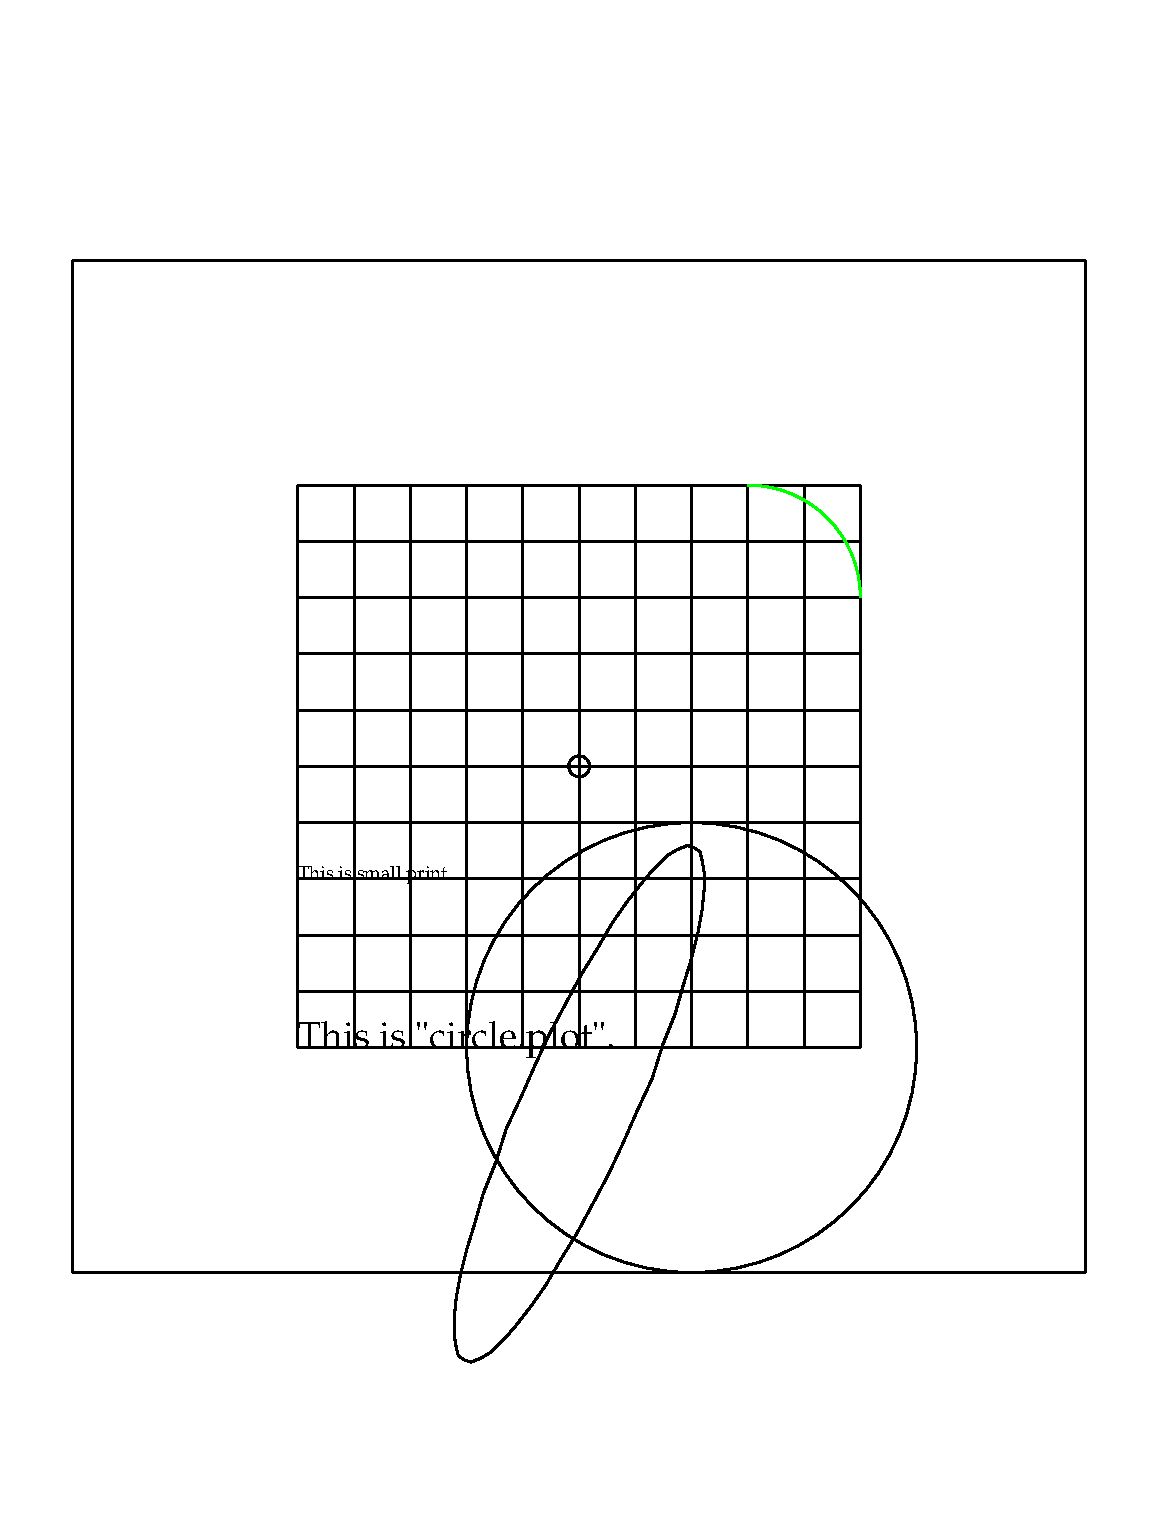
\includegraphics[width=4in]{figure1/figure1.eps}
\end{center}
\caption{
{\bf Foobar.}  Rest of figure 2  caption.  Caption 
should be left justified, as specified by the options to the caption 
package.
}
\label{Figure_label}
\end{figure}

\subsection*{Figure 2}
\begin{figure}[!ht]
\begin{center}
\ifpdf
% \includepdf[pages={1},scale=0.5]{figure2/figure2.pdf}
\includegraphics[width=6in]{figure2/figure2.pdf}
\else
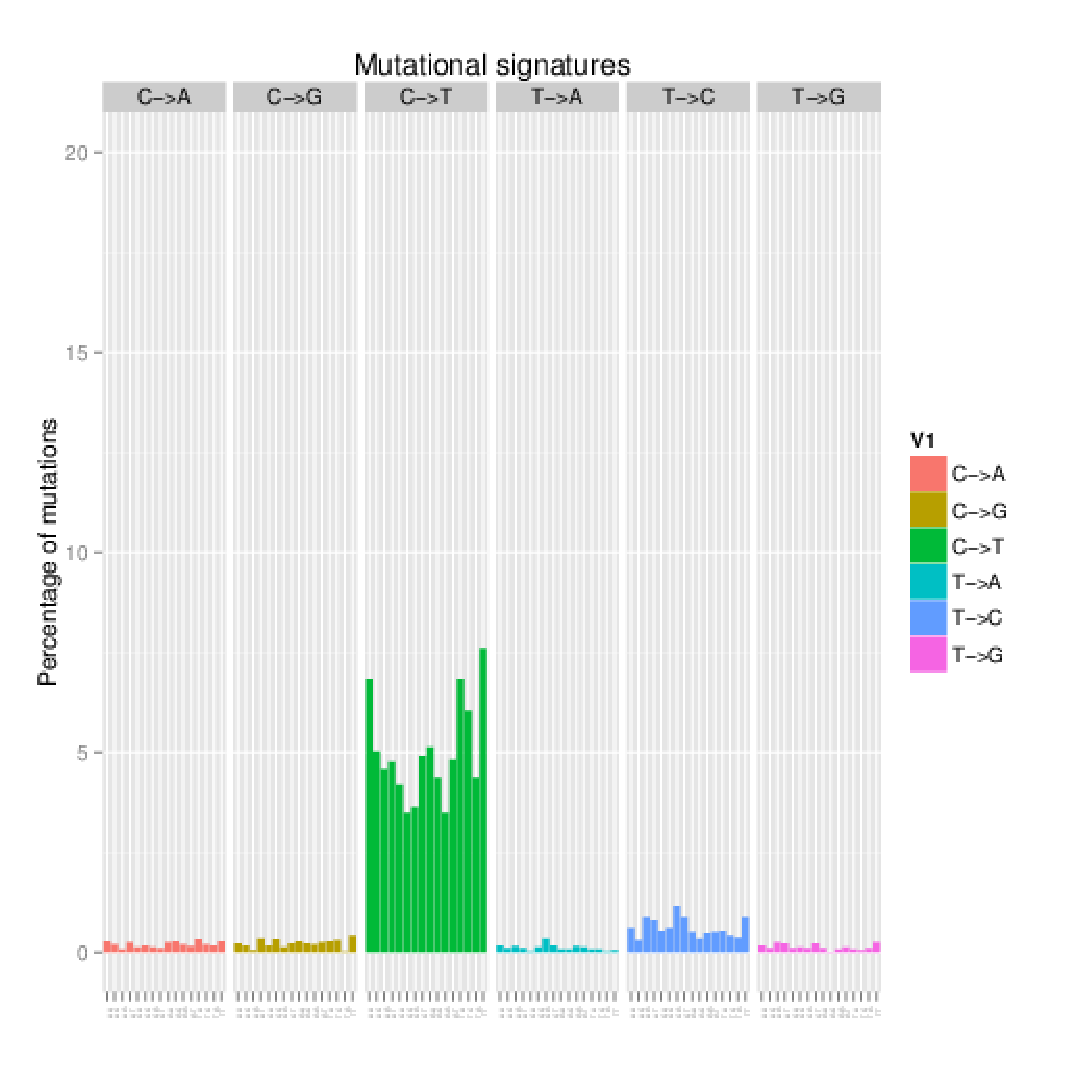
\includegraphics[width=6in]{figure2/mutation_signature.15.30.48_November_05_2013.eps}
\fi
\end{center}
\caption{
{\bf Mutational signature of somatic mutations generated using NPC tumor/normal pair.}  Rest of figure 2  caption.  Caption 
should be left justified, as specified by the options to the caption 
package.
}
\label{Figure_label2}
\end{figure}

\section*{Tables}
%\begin{table}[!ht]
%\caption{
%\bf{Table title}}
%\begin{tabular}{|c|c|c|}
%table information
%\end{tabular}
%\begin{flushleft}Table caption
%\end{flushleft}
%\label{tab:label}
% \end{table}

\end{document}

